\section{Introduction}
\begin{figure}[htbp]
	\centering
	\includegraphics[width=\linewidth]{img/issue/issue}
	\caption{The issue of the self-intersected surface in 3D surface mesh reconstruction networks: (a) A surface mesh of plane generated by Pixel2Mesh\cite{pixel2mesh}. (b) A surface mesh of plane generated by AtlasNet\cite{atlasnet}(sphere as source domain). The triangle faces are rendered as golden on outside and blue on inside. The inside color is exposed due to the issue of self-intersection. Some examples of the issue are also highlighted in zoomed view}
	\label{fig:issue}
\end{figure}
%introduction to 3D shape reconstruction from single view
Inferring 3D shape from a single view image is a traditional problem for computer vision. In computer graphics, 3D modeling with a given image has also been extensively studied. In recent years, deep neural networks (e.g. \cite{3DR2N2,PSGN,3Drender,imgrecon15,3dshapenet,endface,octreegen,surfnet,shapeprior}) have achieved great success in this field. Unlike classic shape from X (e.g. \cite{shapefromshading,shapefromtext1,shapefromtext2}) approaches, these neural networks are able to recover not only the visible frontal shape but also the invisible part for object from a single view color image by learning complicate prior knowledge from dataset. 

These networks all rely on variants of 2D convolution neural network to extract information and encode 2D images, but use quite different techniques to represent and decode 3D shapes. Started by 3D ShapeNets\cite{3dshapenet} and greatly improved by introducing octree structure\cite{octreegen}, volumetric representation and 3D convolution networks are most commonly used in this problem. There is also point set generation network\cite{PSGN} that use unordered point set representation and directly regress point set using both convolution and fully connected branches. Other approaches include \cite{endface} which use bilinear model to represent shape of face and regress the interpolation coefficient to generate the shape and \cite{surfnet} which explicitly employ spherical parameterization as post-processing to represent shape as geometry image in parameter domain and so on.

%introduction to 3d mesh reconstruction networks-- AtlasNet and Pixel2Mesh to be specific
In latest works, AtlasNet\cite{atlasnet} and Pixel2Mesh\cite{pixel2mesh} to be specific, a new idea have been applied on this problem, which let the network learns to map from a predefined surface (square and sphere for AtlasNet and ellipsoid for Pixel2Mesh) to target surface instead of directly regress the absolute positions of surface points as in \cite{PSGN}. These methods have shown great potential in generating meshes for generic objects. It is convenient to integrate mesh-related operations and energy functions in these networks (The graph-based unpooling and Laplacian regularization term from Pixel2Mesh are examples of such integration).

%introduction to the self-intersection issue
In this paper, we address a specific issue that appears in both AtlasNet\cite{atlasnet} and Pixel2Mesh\cite{pixel2mesh}. As shown in Figure~\ref{fig:issue}, the AtlasNet and Pixel2Mesh will generate mesh with self-intersected surface. This issue appears partially because AtlasNet and Pixel2Mesh employed the Chamfer distance loss from point set generation network(PSGN)\cite{PSGN}. The Chamfer distance loss was designed to measure the discrepancy between two unordered point set and it does not take surface into consideration. The AtlasNet used Poission surface reconstruction as post-processing or double-sided lighting in rendering to cover this issue. The Pixel2Mesh have adopted coarse-to-fine framework and added several other losses (i.e. edge length loss, Laplacian loss) that help to alleviate this issue. They all failed to address the essential reason behind this issue, after all this issue is not the central idea of their papers.

In this paper, we focus on the fundamental reason behind this issue, which is that the learned mapping from the predefined surface to target surface is non-injective (as we will show in Sec~\ref{subsec:inj}). In other words, two points on the predefined surface can be mapped to same point by the network causing the generated surface to be self-intersected and self-overlapped. 

%challenge 
Being injective is difficult to enforce and has been studied under parameterization optimization for many years in computer graphics. For surface with disk topology, one possible strategy is to start from a feasible solution (by Tutte's embedding\cite{tutte} or its variants) and keep every optimization iteration or deformation inside feasible region. This can be enforced by adding barrier energy from distortion metrics (e.g. \cite{provableplanarmapping,lifted_bijection}), bounding the triangle distortion (e.g.\cite{freeboundary,boundeddistortion})
or using a progressive strategy\cite{Liu_PP_2018}.
We find it difficult to adopt their strategy in training neural networks, since the network is simultaneously learning to predict the mapping for many different shapes and only a batch of these shapes are sampled from the dataset in each training iteration. It is not easy to use Tutte's embedding to initialize the network or design loss to enforce local injective for batch based optimization. We propose a regularization technique to help enforcing the learning of injective mapping for mesh. Our technique is easy to implement by reusing the existing layers, given an existing surface mesh reconstruction networks as AtlasNet\cite{atlasnet} and Pixel2Mesh\cite{pixel2mesh}.  

\done{have read about some papers about self-intersection removal}
we don't have implementation of this papers, the best we can do is to argue that their strategies are not suitable for training neural networks.
\todo{discuss using self-intersection removal technique as post-process}

%our solution
 Our strategy is to use an additional inverse 3D decoder to learn to predict an inverse mapping from target surface back to the predefined surface along with the forward mapping in the original network. Therefore, a point from predefined surface can be mapped to target surface and then mapped back. We use difference after such cycle mapping to form our regularization term and we call it cycle regularization. While the network learning a mapping to approach the target surface, our regularization term is trying to ensure that an inverse mapping exists (i.e making the forward mapping injective, as we explain in Sec~\ref{subsec:cyclereg}).
Note that the inverse 3D decoder is only needed in training phase, therefore it is only a part of the regularization technique and do not increase the complexity of the original neural network.

In summary, our contributions in this paper are:
\begin{itemize}
	\item We first propose the cycle regularization technique to handle the surface self-intersection for surface mesh reconstruction networks. 
	\item We show that it is simple to implement our cycle regularization technique by applying it on AtlasNet\cite{atlasnet} and Pixel2Mesh\cite{pixel2mesh}. Meanwhile, we also show that our technique keeps the network end-to-end trainable by using existing differentiable layers.
	\item We show that when trained with cycle regularization these networks are able to produce surface meshes with significantly less self-intersection and keep being close to target surface in the sense of Chamfer distance.
\end{itemize}




 